\documentclass[12pt, a4paper]{article}

% Codificacao e idioma
\usepackage[utf8]{inputenc}
\usepackage[T1]{fontenc}
\usepackage[brazil]{babel}

% Layout e margem ABNT
\usepackage[top=3cm, bottom=2cm, left=3cm, right=2cm]{geometry}

% Tipografia
\usepackage{times}
\usepackage{setspace}
\onehalfspacing

% Figuras e tabelas
\usepackage{graphicx}
\usepackage{float}
\usepackage{booktabs}
\usepackage{longtable}
\usepackage{array}
\usepackage{multirow}

% Links e referencias
\usepackage[hidelinks]{hyperref}
\usepackage[
  backend=biber,
  style=abnt,
  citestyle=abnt
]{biblatex}
\addbibresource{referencias.bib}

% Identacao do primeiro paragrafo
\usepackage{indentfirst}

% Melhora quebra de linha e elimina overfull hboxes
\usepackage{microtype}

% Titulos de secao
\setcounter{secnumdepth}{3}

% -----------------------------------------------------------
\begin{document}

% -----------------------------------------------------------
% CABECALHO DO ARTIGO
% -----------------------------------------------------------
\begin{center}
  {\large\bfseries UNIVERSIDADE CAT\'OLICA DE SANTOS}\\[0.2cm]
  {\normalsize Ci\^encia da Computa\c{c}\~ao --- Pesquisa Curricularizada da Gradua\c{c}\~ao}\\[1.4cm]

  {\Large\bfseries Explora+: Detalhamento da Inova\c{c}\~ao, An\'alise de Impacto\\
  e Organiza\c{c}\~ao para o 8\textordmasculine{} Semestre}\\[1.2cm]

  {\normalsize
    Felipe Barbosa dos Santos\quad
    Felipe de Lima Monteiro\quad
    Lucas Carmona Neto\\[0.3cm]
    Lucas Cerqueira Galv\~ao\quad
    Jo\~ao Gabriel Henriques Cardoso
  }\\[0.6cm]

  {\normalsize Santos -- SP, junho de 2026}
\end{center}

\vspace{1.0cm}

% -----------------------------------------------------------
% RESUMO
% -----------------------------------------------------------
\noindent\textbf{Resumo.} O presente artigo constitui a segunda entrega da Pesquisa Curricularizada da Gradua\c{c}\~ao do projeto Explora+, cobrindo quatro eixos: detalhamento das inova\c{c}\~oes t\'ecnicas do prot\'otipo, an\'alise de impacto social, econ\^omico e ambiental, diagrama\c{c}\~ao da solu\c{c}\~ao e planejamento para o 8\textordmasculine{} semestre. O Explora+ \'e um aplicativo m\'ovel para planejamento de rotas tur\'isticas que se distingue pelo uso exclusivo de infraestrutura de dados abertos --- OpenStreetMap, Nominatim, OSRM e Overpass --- eliminando depend\^encia de APIs comerciais e tornando a solu\c{c}\~ao economicamente vi\'avel e replicável em qualquer munic\'ipio com cobertura OSM. As principais inova\c{c}\~oes incluem o enriquecimento progressivo automatizado de pontos de interesse via OSM, Wikidata e Wikip\'edia, o planner multi-POI com cache can\^onico sensível a prefer\^encias individuais, e a personaliza\c{c}\~ao persistente por usu\'ario por meio do modelo \texttt{User\-Route\-Search\-Preference}. A an\'alise de impacto conecta o projeto ao arcabou\c{c}o te\'orico da primeira entrega --- Economia Criativa, Destinos Tur\'isticos Inteligentes e presença digital de estabelecimentos --- e projeta benef\'icios concretos para a popula\c{c}\~ao e para o ecossistema tur\'istico local. O planejamento para o 8\textordmasculine{} semestre organiza o backlog em quatro fases, com a defini\c{c}\~ao do modelo de monetiza\c{c}\~ao como pr\'e-requisito desbloqueador das integra\c{c}\~oes comerciais subsequentes.

\vspace{0.4cm}
\noindent\textbf{Palavras-chave:} Turismo Inteligente. Dados Abertos. OpenStreetMap. Inova\c{c}\~ao Tecnol\'ogica. Planejamento de Produto.

\vspace{0.8cm}

% -----------------------------------------------------------
\section{Introdu\c{c}\~ao}
% -----------------------------------------------------------

A primeira entrega desta pesquisa estabeleceu o arcabou\c{c}o te\'orico que embasa o projeto Explora+: o conceito de Economia Criativa como vetor de desenvolvimento local \parencite{silva2020}, o modelo de Destinos Tur\'isticos Inteligentes (DTI) proposto pelo Minist\'erio do Turismo \parencite{brasil2022}, e evid\^encias emp\'iricas de que a visibilidade digital de pequenos estabelecimentos gera aumento mensur\'avel de receita \parencite{luca2022} e engajamento \parencite{shankar2025}. Sobre essa base, o prot\'otipo funcional foi constru\'ido e entregue, demonstrando a viabilidade t\'ecnica da proposta.

O presente artigo avan\c{c}a para os pr\'oximos eixos exigidos pela disciplina. A \textbf{Se\c{c}\~ao~2} detalha as quatro inova\c{c}\~oes t\'ecnicas centrais do Explora+, com aten\c{c}\~ao especial \`as decis\~oes de arquitetura que as tornam sustent\'aveis e escal\'aveis. A \textbf{Se\c{c}\~ao~3} analisa os impactos social, econ\^omico, educacional e ambiental esperados, conectando-os ao referencial te\'orico j\'a estabelecido. A \textbf{Se\c{c}\~ao~4} apresenta os diagramas que estruturam a solu\c{c}\~ao: componentes, entidade-relacionamento e casos de uso. Por fim, a \textbf{Se\c{c}\~ao~5} organiza o planejamento para o 8\textordmasculine{} semestre, com backlog priorizado, roadmap em quatro fases e requisitos t\'ecnicos que definem a evolu\c{c}\~ao do produto at\'e sua vers\~ao comercial.

% -----------------------------------------------------------
\section{Detalhamento da Inova\c{c}\~ao}
% -----------------------------------------------------------

O Explora+ n\~ao \'e apenas um agregador de pontos de interesse: \'e uma pilha t\'ecnica desenhada para operar sem depend\^encia de APIs comerciais, ao mesmo tempo em que entrega ao usu\'ario uma experi\^encia personalizada e rica em conte\'udo. As quatro subse\c{c}\~oes a seguir detalham cada camada desta inova\c{c}\~ao.

\subsection{Pipeline de Dados Abertos}

A escolha estrat\'egica mais significativa do Explora+ \'e a substitui\c{c}\~ao de APIs comerciais de mapeamento por um \emph{stack} inteiramente composto por projetos abertos e auto-hospedados. A Tabela~\ref{tab:apis} compara as op\c{c}\~oes comerciais originalmente avaliadas com as alternativas adotadas.

\begin{table}[H]
\centering
\caption{Substitui\c{c}\~ao de APIs comerciais por alternativas abertas}
\label{tab:apis}
\small
\begin{tabular}{p{3.8cm}p{3.8cm}p{4.8cm}}
\toprule
\textbf{Fun\c{c}\~ao} & \textbf{API Comercial} & \textbf{Alternativa Adotada} \\
\midrule
Geocodifica\c{c}\~ao de endere\c{c}os & Google Maps Geocoding & Nominatim (OSM) \\
C\'alculo de rotas pedestres & Google Maps Directions & OSRM (Open Source Routing Machine) \\
Descoberta de POIs & GeoAPIFy, Foursquare & Overpass API (OpenStreetMap) \\
Eventos e ingressos & Sympla, TicketMaster & --- (8\textordmasculine{} semestre) \\
Mobilidade urbana & Uber API, 99 API & --- (8\textordmasculine{} semestre) \\
\bottomrule
\end{tabular}
\end{table}

A decis\~ao por dados abertos tem tr\^es motiva\c{c}\~oes complementares. Do ponto de vista \textbf{econ\^omico}, APIs comerciais cobram por volume de requisi\c{c}\~oes: para um aplicativo em escala, o custo opera\c{c}\~onal seria proibitivo antes mesmo da gera\c{c}\~ao de receita. Do ponto de vista \textbf{t\'ecnico}, o OpenStreetMap \parencite{osm2024} \'e a maior base de dados geogr\'aficos colaborativos do mundo, cobrindo mais de 200 pa\'ises com n\'ivel de detalhe superior ao Google Maps em diversas cidades brasileiras. Do ponto de vista de \textbf{soberania de dados}, o projeto n\~ao fica sujeito a mudan\c{c}as unilaterais de pre\c{c}os ou de termos de uso --- problema que afetou in\'umeros projetos em 2018, quando o Google triplicou os pre\c{c}os da Maps Platform.

O Nominatim realiza a convers\~ao de endere\c{c}os em coordenadas geogr\'aficas; o OSRM calcula a rota pedestre \'otima entre os pontos de interesse; e a Overpass API consulta todos os n\'os e rela\c{c}\~oes do OpenStreetMap dentro de um raio configurado pelo usu\'ario, retornando POIs de categorias selecionadas (cultura, parques e natureza, alimenta\c{c}\~ao). O diagrama de componentes da Se\c{c}\~ao~4 ilustra como esses servi\c{c}os se integram na arquitetura do sistema.

\subsection{Enriquecimento Progressivo de POIs}

Dados do OpenStreetMap, embora abrangentes em termos de localiza\c{c}\~ao e categoria, frequentemente carecem de descri\c{c}\~oes, fotografias e conte\'udo editorial sobre os lugares. Para suprir essa lacuna sem curadoria manual --- invi\'avel em escala --- o Explora+ implementa um pipeline de \textbf{enriquecimento progressivo} em tr\^es camadas:

\begin{enumerate}
  \item \textbf{Extratags do OSM:} ao consultar a Overpass API, o sistema coleta todos os campos adicionais do n\'o OSM (\texttt{tourism}, \texttt{name}, \texttt{description}, \texttt{website}, \texttt{phone}, \texttt{opening\_\allowbreak{}hours}). Muitos POIs j\'a possuem estas informa\c{c}\~oes preenchidas pela comunidade.

  \item \textbf{Wikidata (propriedade P18):} se o n\'o OSM cont\'em o campo \texttt{wikidata} com o identificador do local no Wikidata, o sistema consulta automaticamente a propriedade P18 (\textit{image}) para obter a URL de uma fotografia licenciada sob Creative Commons. Esta etapa \'e executada de forma ass\'incrona para n\~ao bloquear a resposta da rota.

  \item \textbf{Wikip\'edia (fallback pt \textrightarrow{} en):} se o n\'o OSM cont\'em o campo \texttt{wikipedia}, o sistema consulta o resumo da p\'agina em portugu\^es. Quando a p\'agina n\~ao existe em portugu\^es, o sistema tenta automaticamente o c\'odigo de idioma em ingl\^es (\textit{fallback}), garantindo que mesmo POIs sem descri\c{c}\~ao em pt-BR n\~ao fiquem sem conte\'udo.
\end{enumerate}

O resultado final \'e um objeto de POI enriquecido entregue ao frontend, com nome, coordenadas, categoria, descri\c{c}\~ao editorial e fotografia --- tudo obtido de fontes abertas, sem curadoria manual e sem custo por requisi\c{c}\~ao. O diagrama de sequ\^encia na Figura~\ref{fig:sequencia} ilustra o fluxo de enriquecimento de um POI individual.

\begin{figure}[H]
  \centering
  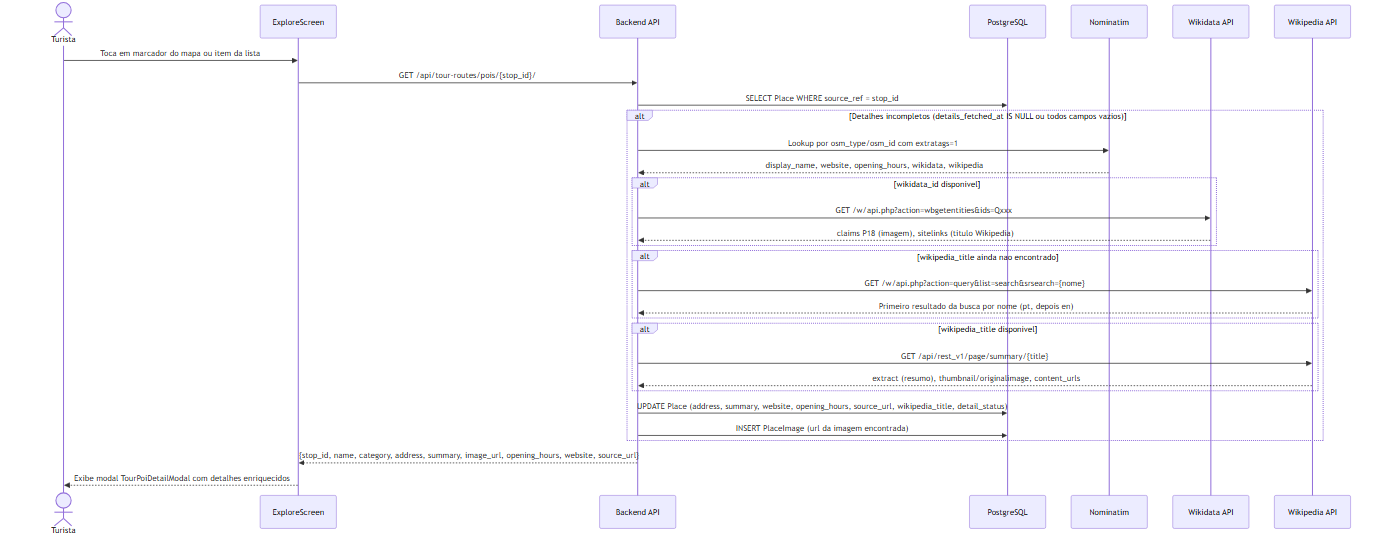
\includegraphics[width=0.90\textwidth]{figuras/sequencia-detalhe-poi.png}
  \caption{Diagrama de sequ\^encia: enriquecimento de detalhe de POI}
  \label{fig:sequencia}
\end{figure}

Esta abordagem \'e inovadora no contexto de aplica\c{c}\~oes tur\'isticas brasileiras: diferente de plataformas como TripAdvisor (que depende de avalia\c{c}\~oes manuais), Google Maps (que depende de fotos enviadas por usu\'arios) ou guias editoriais (que exigem equipes de redatores), o Explora+ extrai conte\'udo j\'a existente em bases colaborativas, sem requerer nenhuma intera\c{c}\~ao humana adicional para cada novo POI inclu\'ido.

\subsection{Planner Multi-POI com Personaliza\c{c}\~ao por Usu\'ario}

O n\'ucleo computacional do Explora+ \'e o planner de rotas, que evoluiu do paradigma de rota com destino \'unico para um planejador multi-POI personalizado. Dado um ponto de partida e um destino final, o sistema:

\begin{enumerate}
  \item Calcula a rota pedestre bruta entre os dois pontos via OSRM;
  \item Consulta todos os POIs no entorno do trajeto, respeitando raio e dist\^ancia entre pontos configurados pelo usu\'ario;
  \item Filtra os POIs pelas categorias habilitadas nas prefer\^encias do usu\'ario;
  \item Ordena os POIs por dist\^ancia ao trajeto, selecionando os mais pr\'oximos;
  \item Recalcula a rota final passando pelos POIs selecionados em ordem.
\end{enumerate}

{\sloppy
O diferencial frente a solu\c{c}\~oes existentes est\'a nos modelos \texttt{User\-Route\-Search\-Preference} e \texttt{Route\-Search\-Cache}. O primeiro persiste, por usu\'ario autenticado, as prefer\^encias de busca: categorias de interesse (\textit{cultura}, \textit{parques}, \textit{alimenta\c{c}\~ao}), dist\^ancia m\'inima entre POIs (75\,m, 100\,m ou 150\,m) e raio m\'aximo de busca em torno do trajeto (150\,m, 250\,m ou 400\,m). O segundo implementa um cache inteligente cujo identificador (\textit{cache key}) incorpora as prefer\^encias do usu\'ario: dois usu\'arios com prefer\^encias diferentes para o mesmo trajeto obter\~ao rotas distintas, enquanto o mesmo usu\'ario que repetir uma busca id\^entica recebe o resultado em milissegundos, sem re-executar as consultas \`a Overpass API e ao OSRM.
\par}

Esta combina\c{c}\~ao de personaliza\c{c}\~ao e cache \'e especialmente relevante para o turismo: visitantes que preferem gastronomia e aqueles que preferem hist\'oria e cultura merecem itiner\'arios diferentes, mesmo que partam e cheguem ao mesmo ponto. A personaliza\c{c}\~ao por usu\'ario \'e o que diferencia o Explora+ de um simples visualizador de pontos no mapa.

\subsection{Plataforma Transfer\'ivel para Qualquer Munic\'ipio}

Uma decis\~ao de arquitetura impl\'icita nas escolhas anteriores merece destaque expl\'icito: o Explora+ n\~ao est\'a acoplado a Santos~--~SP. A configura\c{c}\~ao do ponto de busca \'e din\^amica e determinada pelas coordenadas fornecidas pelo usu\'ario no frontend; o backend n\~ao cont\'em nenhuma refer\^encia geogr\'afica \emph{hardcoded}.

Para implantar o Explora+ em outra cidade, basta:
\begin{itemize}
  \item Garantir que a cidade tenha cobertura no OpenStreetMap (v\'alido para praticamente todos os munic\'ipios brasileiros e para mais de 200 pa\'ises);
  \item Atualizar os dados de semente (\textit{seed}) com pontos de interesse curados localmente (opcional, pois o discovery via Overpass j\'a funciona sem seeds);
  \item Configurar a vari\'avel de ambiente de URL do backend no frontend.
\end{itemize}

Esta transferibilidade tem impacto direto no potencial de escala do projeto. Enquanto guias tur\'isticos tradicionais s\~ao produzidos por cidade, o Explora+ \'e uma infraestrutura reutiliz\'avel que pode ser implantada por prefeituras, secretarias de turismo ou grupos acad\^emicos em qualquer localidade, conforme discutido na Se\c{c}\~ao~3.

% -----------------------------------------------------------
\section{An\'alise de Impacto}
% -----------------------------------------------------------

A primeira entrega desta pesquisa identificou tr\^es eixos de impacto potencial: a visibilidade digital de pequenos estabelecimentos \parencite{luca2022,shankar2025}, a experi\^encia do visitante como vetor de Economia Criativa \parencite{silva2020,melo2022}, e o modelo de Destinos Tur\'isticos Inteligentes como referencial de pol\'itica p\'ublica \parencite{brasil2022}. Com o prot\'otipo constru\'ido, \'e poss\'ivel agora analisar esses impactos com maior especificidade.

\subsection{Impacto Social}

O principal impacto social do Explora+ \'e a \textbf{democratiza\c{c}\~ao da descoberta tur\'istica}. Visitantes e pr\'oprios moradores de Santos frequentemente desconhecem uma parcela significativa do patrim\^onio cultural, natural e gastron\^omico dispon\'ivel na cidade. O aplicativo resolve esse problema de duas formas complementares:

Primeiro, ao calcular rotas que passam por POIs pr\'oximos ao trajeto do usu\'ario, o Explora+ expande naturalmente o horizonte do visitante para al\'em dos pontos mais famosos --- o efeito de descoberta (\textit{serendipity}) \'e embutido no algoritmo, n\~ao dependendo de busca ativa do usu\'ario.

Segundo, ao agregar conte\'udo editorial proveniente do Wikidata e da Wikip\'edia, o aplicativo oferece contexto hist\'orico e cultural sobre cada ponto visitado, transformando um passeio recreativo em uma experi\^encia educativa acess\'ivel.

Para estabelecimentos com menor visibilidade digital --- cafeterias, galerias de arte alternativas, parques municipais --- o Explora+ funciona como um \textit{aggregator} de visibilidade gratuito. \textcite{luca2022} demonstraram que a presen\c{c}a em plataformas digitais gera incremento m\'edio de 5\% na receita de pequenos neg\'ocios, especialmente aqueles sem or\c{c}amento para marketing tradicional. O Explora+ replica esse efeito para estabelecimentos que sequer t\^em perfil no Google Maps ou no TripAdvisor, desde que existam no OpenStreetMap.

\subsection{Impacto Econ\^omico}

O impacto econ\^omico do Explora+ opera em dois n\'iveis distintos.

No n\'ivel \textbf{micro}, o aplicativo amplia o alcance de clientes para estabelecimentos locais ao inclu\'i-los organicamente nas rotas geradas. Um restaurante no centro hist\'orico que n\~ao investe em publicidade passa a ser sugerido a turistas cujas rotas passam pr\'oximas a ele. Esta amplifica\c{c}\~ao de visibilidade segue o mesmo mecanismo documentado por \textcite{shankar2025} para o Google Business Profile, mas sem requerer que o estabelecimento gerencie ativamente seu perfil digital.

No n\'ivel \textbf{macro}, o aplicativo contribui para a \textbf{descentraliza\c{c}\~ao do fluxo tur\'istico}. Cidades tur\'isticas sofrem frequentemente do fen\^omeno de \textit{overtourism}: a concentra\c{c}\~ao de visitantes em poucos pontos famosos ao mesmo tempo em que \'areas igualmente interessantes permanecem subutilizadas. Ao distribuir rotas por m\'ultiplos POIs em diferentes bairros, o Explora+ fomenta um turismo mais distribu\'ido geograficamente, com benef\'icios econ\^omicos para mais estabelecimentos.

Para o pr\'oprio produto, o modelo de monetiza\c{c}\~ao discutido na Se\c{c}\~ao~5 prev\^e tr\^es fontes de receita: POIs patrocinados (estabelecimentos que pagam para ser destacados nas rotas), planos premium (funcionalidades avan\c{c}adas para usu\'arios recorrentes) e parcerias com ag\^encias e operadoras de turismo.

\subsection{Impacto Educacional e Extensionista}

O Explora+ \'e um projeto de extens\~ao universit\'aria, e esse car\'ater determina uma dimens\~ao de impacto freq\"uentemente negligenciada em an\'alises de produto: o \textbf{impacto sobre o pr\'oprio processo de desenvolvimento}.

A equipe enfrentou e resolveu problemas reais e complexos: integra\c{c}\~ao de bases de dados geogr\'aficas heterog\^eneas, implementa\c{c}\~ao de cache distribu\'ido com chaves compostas, desenvolvimento mobile com Expo e React Native, e entrega de um sistema de ponta a ponta com autenticac\~ao, persist\^encia e rotas calculadas em produc\~ao. Nenhum desses problemas seria encontrado em um projeto puramente acad\^emico com dados sint\'eticos.

Al\'em disso, toda a base de c\'odigo est\'a publicada sob licen\c{c}a aberta na organiza\c{c}\~ao EXPLORA-PLUS no GitHub\footnote{\url{https://github.com/EXPLORA-PLUS}}, permitindo que outros grupos acad\^emicos, secretarias municipais ou desenvolvedores independentes utilizem, adaptem e ampliem o projeto. Esta transferibilidade amplifica o impacto educacional muito al\'em do grupo original.

\subsection{Impacto Ambiental}

O Explora+ \'e concebido como um aplicativo de \textbf{rotas pedestres}. Diferente de plataformas que integram taxi, carro por aplicativo ou ve\'iculos pr\'oprios como modal padr\~ao, o Explora+ planeja itiner\'arios que o usu\'ario percorre a p\'e.

Este foco tem um impacto ambiental direto e mensur\'avel: cada quilômetro percorrido a p\'e em vez de carro representa aproximadamente 170\,g de CO$_2$ n\~ao emitidos (considerando a m\'edia de emiss\~ao de ve\'iculos leves no Brasil). Para um turista que visita 5 POIs distribu\'idos em 3\,km de percurso --- cen\'ario t\'ipico no centro hist\'orico de Santos ---, a substitui\c{c}\~ao do deslocamento de carro pelo trajeto a p\'e evita cerca de 500\,g de CO$_2$ por visita.

Ademais, a promos\~ao do turismo pedestre em centros hist\'oricos contribui para a vitalidade urbana: ruas mais movimentadas a p\'e geram maior seguran\c{c}a percebida, maior consumo no com\'ercio local e melhor qualidade de vida para moradores --- um conjunto de externalidades positivas amplamente documentado na literatura de urbanismo.

% -----------------------------------------------------------
\section{Diagramas}
% -----------------------------------------------------------

Esta se\c{c}\~ao apresenta os tr\^es diagramas centrais da arquitetura do Explora+. Diferente da documenta\c{c}\~ao t\'ecnica do projeto, a leitura aqui \'e orientada pelas inova\c{c}\~oes descritas na Se\c{c}\~ao~2 e pelos impactos analisados na Se\c{c}\~ao~3.

\subsection{Arquitetura de Componentes}

\begin{figure}[H]
  \centering
  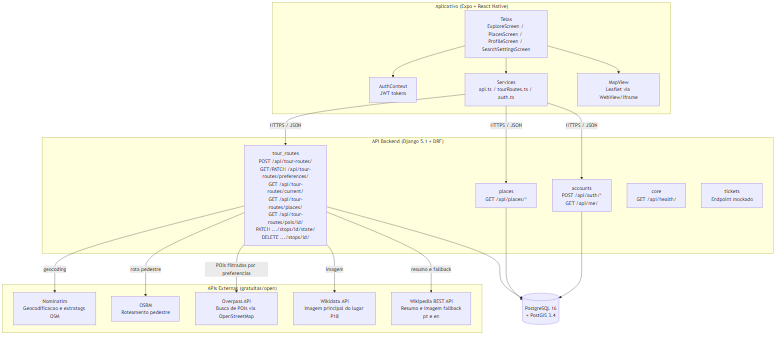
\includegraphics[width=\textwidth]{figuras/componentes.png}
  \caption{Diagrama de componentes da arquitetura Explora+}
  \label{fig:componentes}
\end{figure}

O diagrama da Figura~\ref{fig:componentes} evidencia a separa\c{c}\~ao clara entre tr\^es camadas: o frontend m\'ovel (Expo/React Native), o backend Django com seus servi\c{c}os especializados (Geocoding, Routing, Overpass, Wikidata, Wikipedia, MapBuilder) e as fontes de dados externas (Nominatim, OSRM, Overpass API, Wikidata, Wikip\'edia). Nenhuma das fontes externas \'e comercial: todas s\~ao projetos de dados abertos ou APIs p\'ublicas sem custo por requisi\c{c}\~ao.

O componente \texttt{MapBuilder} coordena o pipeline descrito na Se\c{c}\~ao~2.2: recebe os POIs brutos do Overpass, delega o enriquecimento aos servi\c{c}os de Wikidata e Wikip\'edia, e monta o objeto de rota enriquecido que ser\'a persistido no banco de dados e entregue ao frontend.

\subsection{Modelo Entidade-Relacionamento}

\begin{figure}[H]
  \centering
  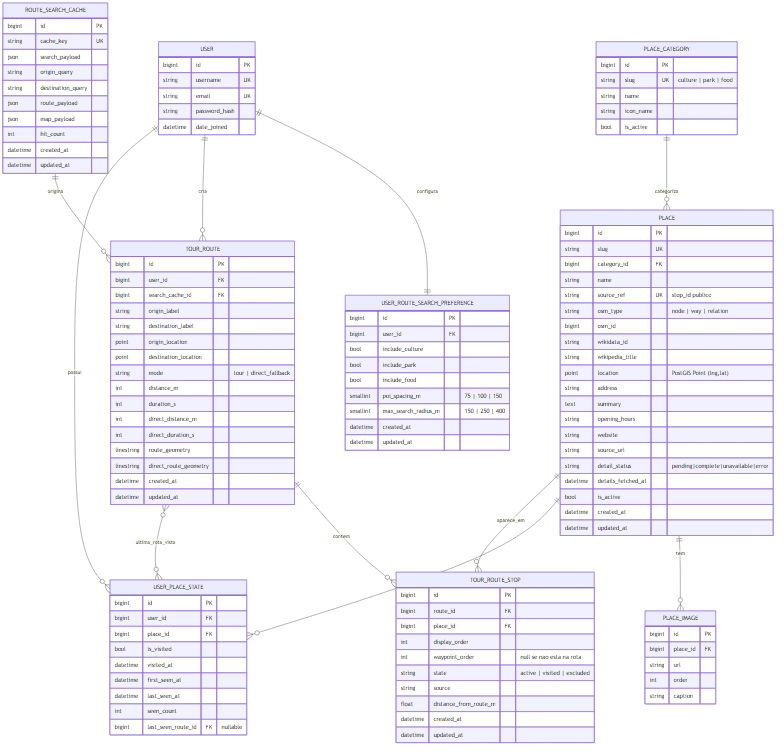
\includegraphics[width=\textwidth, keepaspectratio]{figuras/er.png}
  \caption{Diagrama entidade-relacionamento do banco de dados Explora+}
  \label{fig:er}
\end{figure}

O modelo da Figura~\ref{fig:er} reflete as inova\c{c}\~oes descritas na Se\c{c}\~ao~2.3. As entidades \texttt{User\-Route\-Search\-Preference} e \texttt{Route\-Search\-Cache} s\~ao o corac\~ao da personaliza\c{c}\~ao: a primeira associa ao usu\'ario autenticado um conjunto de prefer\^encias que determinam os par\^ametros de busca; a segunda armazena rotas calculadas com uma chave can\^onica que incorpora essas prefer\^encias, evitando recalculos desnecess\'arios.

As entidades \texttt{Place} e \texttt{PlaceImage} sustentam o cat\'alogo de POIs curados manualmente, que coexiste com o discovery din\^amico via Overpass. A tabela \texttt{RouteStop} vincula cada parada de uma rota calculada a seu POI correspondente, armazenando o estado de visita\c{c}\~ao (\textit{visited}, \textit{skipped}) para permitir acompanhamento da progress\~ao da rota pelo usu\'ario.

\subsection{Casos de Uso}

\begin{figure}[H]
  \centering
  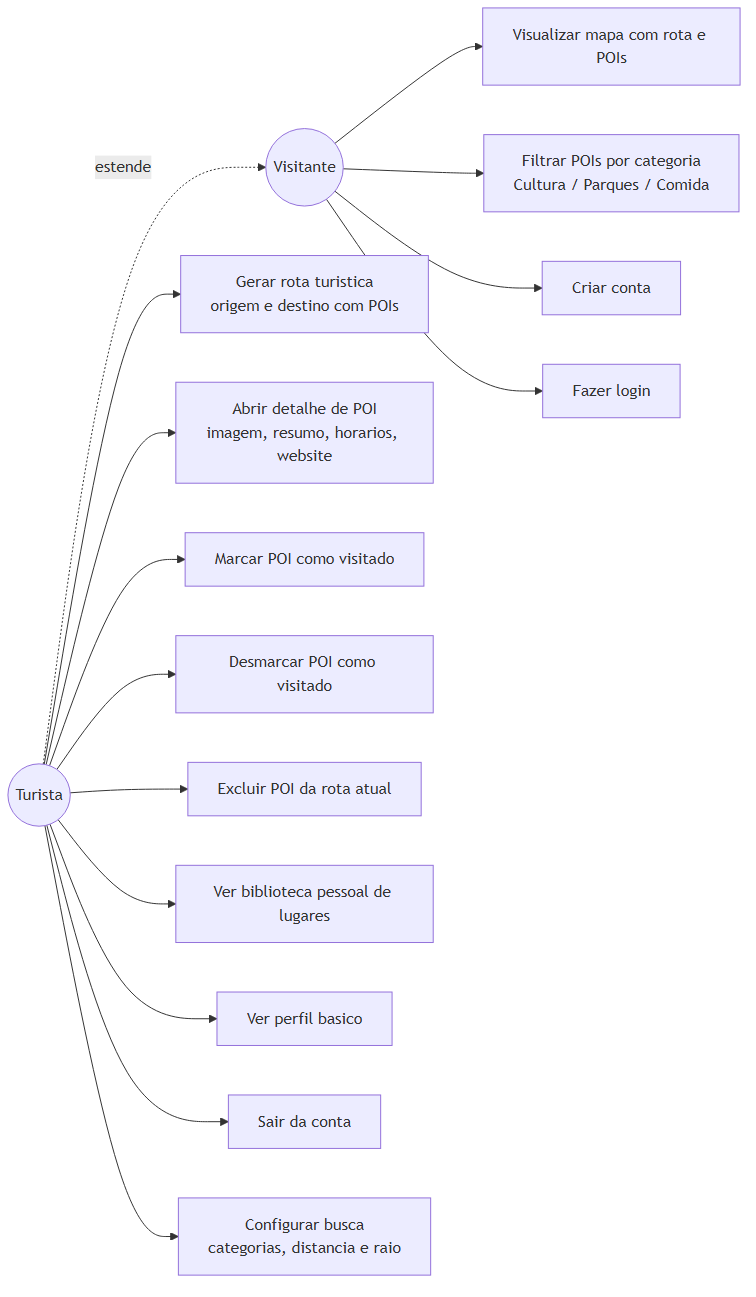
\includegraphics[height=0.72\textheight, keepaspectratio]{figuras/casos-de-uso.png}
  \caption{Diagrama de casos de uso do Explora+}
  \label{fig:casosdeuso}
\end{figure}

O diagrama de casos de uso da Figura~\ref{fig:casosdeuso} delimita o escopo de intera\c{c}\~ao do usu\'ario com o sistema. Tr\^es grupos de casos de uso mapeiam diretamente para as inova\c{c}\~oes descritas:

\begin{itemize}
  \item \textbf{Gerar rota personalizada} encapsula o planner multi-POI com prefer\^encias da Se\c{c}\~ao~2.3;
  \item \textbf{Visualizar detalhe de POI} exprime o enriquecimento progressivo da Se\c{c}\~ao~2.2;
  \item \textbf{Configurar prefer\^encias de busca} torna vis\'ivel para o usu\'ario o mecanismo de personaliza\c{c}\~ao que alimenta o cache.
\end{itemize}

O ator \emph{Sistema Externo} representa o conjunto de APIs abertas (Nominatim, OSRM, Overpass, Wikidata, Wikip\'edia), evidenciando que a maior parte da intelig\^encia do aplicativo reside na integra\c{c}\~ao dessas fontes, n\~ao em dados propriet\'arios.

% -----------------------------------------------------------
\section{Organiza\c{c}\~ao para o 8\textordmasculine{} Semestre}
% -----------------------------------------------------------

O prot\'otipo entregue demonstra a viabilidade t\'ecnica da proposta e valida as hip\'oteses centrais do projeto. Para evoluir de um prot\'otipo acad\^emico para um produto com potencial comercial e impacto de escala, o 8\textordmasculine{} semestre deve cumprir um conjunto espec\'ifico de objetivos. Esta se\c{c}\~ao estrutura esse caminho.

\subsection{Pr\'e-requisito: Defini\c{c}\~ao do Modelo de Monetiza\c{c}\~ao}

Antes de iniciar qualquer integra\c{c}\~ao comercial, o grupo precisa definir \textbf{como o Explora+ gera receita}. Esta decis\~ao n\~ao \'e apenas estrat\'egica: ela determina quais integrações t\'ecnicas s\~ao prioritárias e condiciona as negociac\~oes com parceiros.

Tr\^es modelos s\~ao vi\'aveis e n\~ao mutuamente exclusivos:

\begin{enumerate}
  \item \textbf{POI patrocinado:} estabelecimentos pagam para ser priorizados nas rotas geradas para usu\'arios que passam pr\'oximos. Requer defini\c{c}\~ao de modelo de precifica\c{c}\~ao (CPC, CPM ou assinatura) e interface de gest\~ao para o estabelecimento.

  \item \textbf{Plano premium:} usu\'arios pagam por funcionalidades avan\c{c}adas --- rotas sem limite de POIs, hist\'orico de rotas ilimitado, exporta\c{c}\~ao para GPS, modo offline. Requer integra\c{c}\~ao com gateway de pagamento (Stripe ou Pagar.me).

  \item \textbf{Parceria B2B:} ag\^encias de turismo e secretarias municipais licenciam a plataforma para distribuir roteiros oficiais. Requer interface de administra\c{c}\~ao e API de curadoria.
\end{enumerate}

A defini\c{c}\~ao deste modelo no in\'icio do 8\textordmasculine{} semestre \'e o pr\'e-requisito que desbloqueia as fases subsequentes.

\subsection{Backlog Priorizado}

A Tabela~\ref{tab:backlog} organiza o backlog de funcionalidades para o 8\textordmasculine{} semestre por prioridade, depend\^encia e esfor\c{c}o estimado.

\begin{table}[H]
\centering
\caption{Backlog priorizado para o 8\textordmasculine{} semestre}
\label{tab:backlog}
\begin{tabular}{p{5.5cm}ccc}
\toprule
\textbf{Funcionalidade} & \textbf{Prioridade} & \textbf{Depende de} & \textbf{Esfor\c{c}o} \\
\midrule
Defini\c{c}\~ao do modelo de monetiza\c{c}\~ao & Alta & --- & M\'edio \\
Integra\c{c}\~ao Sympla / Ticketmaster & Alta & Monetiza\c{c}\~ao & Alto \\
POI patrocinado (backend + admin) & Alta & Monetiza\c{c}\~ao & Alto \\
Gateway de pagamento (plano premium) & M\'edia & Monetiza\c{c}\~ao & Alto \\
Integra\c{c}\~ao Uber / 99 & M\'edia & Monetiza\c{c}\~ao & M\'edio \\
Transporte p\'ublico (GTFS) & M\'edia & API p\'ublica & M\'edio \\
Notifica\c{c}\~oes push (POIs pr\'oximos) & M\'edia & --- & Baixo \\
Avalia\c{c}\~oes e fotos pela comunidade & M\'edia & --- & M\'edio \\
Edi\c{c}\~ao de perfil do usu\'ario & Baixa & --- & Baixo \\
Busca por voz & Baixa & --- & M\'edio \\
Painel admin (curadoria de POIs) & Baixa & --- & Baixo \\
\bottomrule
\end{tabular}
\end{table}

\subsection{Fases Propostas}

O 8\textordmasculine{} semestre \'e dividido em quatro fases de quatro semanas cada, com entregas progressivas:

\textbf{Fase 1 --- Fundamentos Comerciais (semanas 1--4):} Defini\c{c}\~ao e valida\c{c}\~ao do modelo de monetiza\c{c}\~ao com \textit{stakeholders}; implementa\c{c}\~ao da integra\c{c}\~ao com Sympla e/ou Ticketmaster para eventos; prototipagem do mecanismo de POI patrocinado no backend. Entrega: Explora+ com eventos reais e primeiro modelo comercial definido.

\textbf{Fase 2 --- Mobilidade e Engajamento (semanas 5--8):} Integra\c{c}\~ao com Uber API e/ou GTFS para transporte p\'ublico; implementa\c{c}\~ao de notifica\c{c}\~oes push para POIs pr\'oximos; conclus\~ao do gateway de pagamento para plano premium. Entrega: Explora+ com mobilidade integrada e plano premium operacional.

\textbf{Fase 3 --- Comunidade e Escala (semanas 9--12):} Sistema de avalia\c{c}\~oes e fotos pela comunidade; configura\c{c}\~ao para implanta\c{c}\~ao em nova cidade-piloto (al\'em de Santos); painel de administra\c{c}\~ao para curadoria de POIs. Entrega: Explora+ com features sociais e segunda cidade ativa.

\textbf{Fase 4 --- Consolida\c{c}\~ao (semanas 13--16):} Testes de carga, refatora\c{c}\~ao de gargalos identificados, aplica\c{c}\~ao de feedback dos usu\'arios das fases anteriores, documenta\c{c}\~ao final e apresenta\c{c}\~ao do produto. Entrega: vers\~ao est\'avel e demonstr\'avel para banca e parceiros.

\subsection{Requisitos T\'ecnicos para o 8\textordmasculine{} Semestre}

A evolu\c{c}\~ao descrita nas fases anteriores exige os seguintes requisitos t\'ecnicos que n\~ao est\~ao presentes no prot\'otipo atual:

\begin{itemize}
  \item \textbf{Backend:} \textit{adapters} isolados para as APIs da Sympla e do Ticketmaster, com tratamento de autentica\c{c}\~ao OAuth2 e \textit{rate limiting}; integra\c{c}\~ao com GTFS para leitura de dados de transporte p\'ublico; endpoint de gest\~ao de POIs patrocinados com painel administrativo; integra\c{c}\~ao com gateway de pagamento (Stripe ou Pagar.me) para gest\~ao de assinaturas.

  \item \textbf{Frontend:} sistema de notifica\c{c}\~oes push via Expo Notifications; tela de avalia\c{c}\~oes e upload de fotos; tela de edi\c{c}\~ao de perfil; indica\c{c}\~ao visual de POIs patrocinados na interface de rota; integra\c{c}\~ao com deep linking para abertura direta de apps de mobilidade (Uber, 99).

  \item \textbf{Infraestrutura:} vari\'aveis de ambiente para gest\~ao segura de chaves de APIs comerciais; monitora\c{c}\~ao de erros em produ\c{c}\~ao (Sentry ou equivalente); estrat\'egia de \textit{cache} para respostas de APIs de eventos (que mudam com frequ\^encia di\'aria).
\end{itemize}

% -----------------------------------------------------------
\section{Conclus\~ao}
% -----------------------------------------------------------

Este artigo detalhou as quatro inova\c{c}\~oes centrais do Explora+ --- o pipeline de dados abertos, o enriquecimento progressivo de POIs, o planner multi-POI com personaliza\c{c}\~ao por usu\'ario e a arquitetura transfer\'ivel para qualquer munic\'ipio ---, analisou os impactos social, econ\^omico, educacional e ambiental esperados, e estruturou o planejamento para a evolu\c{c}\~ao do produto no 8\textordmasculine{} semestre.

A inova\c{c}\~ao do Explora+ n\~ao reside em nenhuma t\'ecnica singular, mas na combina\c{c}\~ao de tr\^es elementos que raramente coexistem em aplica\c{c}\~oes tur\'isticas: dados inteiramente abertos, personaliza\c{c}\~ao por usu\'ario e transferibilidade geogr\'afica sem custo incremental. Essa combina\c{c}\~ao torna o projeto economicamente vi\'avel onde solu\c{c}\~oes baseadas em APIs comerciais n\~ao seriam, e socialmente relevante onde plataformas globais n\~ao chegam com profundidade local.

O 8\textordmasculine{} semestre representa a transi\c{c}\~ao do prot\'otipo acad\^emico para produto com potencial de impacto real. A base t\'ecnica est\'a constru\'ida e validada; o caminho para a escala comercial passa pela defini\c{c}\~ao do modelo de monetiza\c{c}\~ao e pelas integra\c{c}\~oes de eventos e mobilidade que trar\~ao ao Explora+ a completude necess\'aria para competir com solu\c{c}\~oes estabelecidas. O projeto demonstra que \'e poss\'ivel construir, em contexto universit\'ario, tecnologia com qualidade de produto e impacto de extens\~ao --- sem abrir m\~ao de nenhum dos dois.

% -----------------------------------------------------------
\printbibliography[title={Refer\^encias}]
% -----------------------------------------------------------

\end{document}
